	\chapter{}
\label{lecture10}
\section[Квадратичный функционал. Оператор Шредингера.]{Квадратичный функционал в случае функций, зависящих от нескольких переменных. Оператор Шредингера.}
\label{lecture10section1}
Для функционалов, зависящих от функций нескольких переменных, можно ставить изопериметрические задачи аналогично ситуации с функционалом от функций одной переменной. Однако мы не будем это делать в общем случае, а ограничимся случаем \emph{квадратичных} функционалов для функций трёх переменных
\begin{equation}\label{l10:eq:0}
	\hfill B[u]=\iiint\limits_{\Omega}\left(u_x^2+u_y^2+u_z^2+P(x,y,z)\cdot u^2\right)\,d\Omega,\hfill
\end{equation}
где $u=u(x,y,z)$, $P(x,y,z)\in\Cfn{}(\overline{\Omega})$, $\Omega$ --- ограниченная область в $\R^3$. Минимум $B[u]$ ищем в классе
\begin{equation*}
	\hfill\K=\left\{u(x,y,z)|u\in\Cfn{1}(\overline{\Omega}),\ u\Big|_{\partial\Omega}=0,\ \iiint\limits_{\Omega}u^2\,d\Omega=1\right\}_{\displaystyle.}\hfill
\end{equation*}

Повторяя рассуждения, проведённые для изопериметрических задач в случае $\J[y]$, $y=y(x)$, мы получим, что минимайзер в задаче на $\displaystyle\min\limits_{u\in\K}B[u]$ удовлетворяет уравнению Пуассона для интегранта
\begin{equation*}
	\hfill F^{\ast}=F-\lambda\cdot u^2=u_x^2+u_y^2+u_z^2+P\cdot u^2-\lambda\cdot u^2,\hfill
\end{equation*}
и, значит,  уравнение Пуассона можно записать в виде
\begin{equation}\label{l10:eq:1}
	\hfill-\Delta u+P\cdot u=\lambda\cdot u\qquad\qquad\left(\Delta\eqdef\pdder{}{x}+\pdder{}{y}+\pdder{}{z}\right).\hfill
\end{equation}
Оператор $H=-\Delta+P$ называется оператором Шредингера, при $P=0$ --- оператором Лапласа. Мы рассматриваем функцию $3^{\text{ёх}}$ переменных, но можно рассматривать двух и вообще $n$. Решение~\eqref{l10:eq:1} ищется в классе функций $u\in\Cfn{2}(\Omega)\cap\Cfn{1}(\overline{\Omega})$, $u\Big|_{S}=0$ и $S=\partial\Omega$. Таким образом, минимайзер является собственной функцией оператора Шредингера, отвечающей собственному значению $\lambda$. Докажем эрмитовость оператора $H$ в $\Cfn{2}(\Omega)\cap\Cfn{1}(\overline{\Omega})$ при заданном условии $u\Big|_{S}=0$ и при других возможных граничных условиях (аналогичных тем, что были в одномерной ситуации.)
\begin{equation}\label{l10:eq:A}
	\hfill u\Big|_{S}=0;\tag{A}\hfill
\end{equation}
\begin{equation}\label{l10:eq:B}
	\hfill \left(\pder{u}{n}+\gamma\cdot u\middle)\right|_{S}=0,\quad\gamma\geqslant0;\tag{B}\hfill
\end{equation}
где $u\in\Cfn{2}(\Omega)\cap\Cfn{1}(\overline{\Omega})$.

Мы рассматриваем оператор Шредингера в пространстве 
\begin{equation*}
	\hfill\fL[(\Omega)]=\left\{u(x,y,z)\middle|\iiint\limits_{\Omega}|u|^2\,d\Omega<+\infty\right\}_{\displaystyle.}\hfill
\end{equation*}
При $u,v\in\fL[(\Omega)]$ полагаем $\displaystyle\big(u,v\big)\eqdef\iiint\limits_{\Omega}u\cdot\overline{v}\,d\Omega$. Оператор $H$ определим на $\Cfn{2}(\Omega)\cap\Cfn{1}(\overline{\Omega})$ с граничным условием~\eqref{l10:eq:A} или~\eqref{l10:eq:B}. Нам надо доказать, что при $u,\ v\in\mc{D}_{H}$ (область определения)
\begin{equation}\label{l10:eq:2}
	\hfill\big(Hu,v\big)=\big(u,Hv\big).\hfill
\end{equation}
Так как в выражении $H$ (см.~\eqref{l10:eq:1}) функция $P$ --- вещественна, то для справедливости~\eqref{l10:eq:2} достаточно проверить равенство
\begin{equation}\label{l10:eq:3}
	\hfill\big(-\Delta u,v\big)=\big(u,-\Delta v\big).\hfill
\end{equation}
Имеем, выделяя дивергенцию вектора $\bm{\Phi}=(u_x\cdot\overline{v},u_y\cdot\overline{v},u_z\cdot\overline{v})$
\begin{multline}\label{l10:eq:4}
	\big(-\Delta u,v\big)=-\iiint\limits_{\Omega}(u_{xx}+u_{yy}+u_{zz})\cdot\overline{v}\,d\Omega=-\iiint\limits_{\Omega}\underbrace{\left(\pder{}{x}\big(u_x\cdot\overline{v}\big)+\pder{}{y}\big(u_y\cdot\overline{v}\big)+\pder{}{z}\big(u_z\cdot\overline{v}\big)\right)}_{\Div\bm{\Phi}}\,d\Omega+\\
	+\iiint\limits_{\Omega}(u_x\cdot\overline{v}_x+u_y\cdot\overline{v}_y+u_z\cdot\overline{v}_z)\,d\Omega=\iiint\limits_{\Omega}\big(\nabla u,\nabla v\big)_{\R^3}\,d\Omega-\iint\limits_{S}\big(\bm{\Phi},\bm{n}\big)_{\R^3}\,dS,
\end{multline}
где $\bm{n}$ --- единичная внешняя нормаль к $S$: $\bm{n}=(\cos\alpha,\cos\beta,\cos\gamma)$\footnote{Мы применили здесь формулу Остроградского--Гаусса, и именно для этого потребовали $u,\ v\in\Cfn{1}(\overline{\Omega})$. Кроме того, требование $u,\ v\in\Cfn{1}(\overline{\Omega})$ обязательно при условии~\eqref{l10:eq:B} на границе.}. %
В силу~\eqref{l10:eq:4}
\begin{equation}\label{l10:eq:5}
	\big(-\Delta u,v\big)=\iiint\limits_{\Omega}\big(\nabla u,\nabla v\big)_{\R^3}\,d\Omega-\iint\limits_{S}\pder{u}{n}\cdot\overline{v}\,dS.
\end{equation}
Далее
\begin{equation}\label{l10:eq:6}
	-\big(u,\Delta v\big)=-\overline{\big(\Delta v,u\big)}=\overline{\iiint\limits_{\Omega}\big(\nabla v,\nabla u\big)_{\R^3}\,d\Omega}-\iint\limits_{S}\pder{\overline{v}}{n}\cdot u\,dS.
\end{equation}
Таким образом для эрмитовости оператора лапласа надо, чтобы на границе $S$
\begin{equation*}
	\hfill\pder{u}{n}\cdot\overline{v}=\pder{\overline{v}}{n}\cdot u.\hfill
\end{equation*}
При условии~\eqref{l10:eq:A} получаем, что $0=0$, а при условии~\eqref{l10:eq:B} получаем, что $-\gamma\cdot u\cdot\overline{v}=-\overline{\gamma}\cdot\overline{v}\cdot u$\footnote{На части $S$ может выполняться~\eqref{l10:eq:A}, на части~\eqref{l10:eq:B} --- рассуждения сохраняются.}. Таким образом при вещественном $\gamma$ оператора $\Delta$ эрмитов в случае условия~\eqref{l10:eq:B}, а при $\gamma$ --- комплексном --- нет. Кроме того, заметим, что при условии~\eqref{l10:eq:A} при $u=v$
\begin{equation}\label{l10:eq:7}
	\hfill\big(Hu,u\big)=B[u],\hfill
\end{equation} 
а при условии~\eqref{l10:eq:B}
\begin{equation}\label{l10:eq:8}
	\hfill\big(Hu,u\big)=\widetilde{B}[u]\eqdef\iiint\limits_{\Omega}\left(\left|\nabla u\right|^2+P\cdot|u|^2\right)\,d\Omega+\gamma\cdot\iint\limits_{S}|u|^2\,dS.\hfill
\end{equation}
В силу эрмитовости оператора $H$ замечаем, что собственные значения $H$ --- вещественны и собственные функции, отвечающие различным собственным значениям, взаимно ортогональны (как и для оператора Штурма). Однако по сравнению с ним есть существенное отличие. Кроме наименьшего собственного значения оператора $H$ все остальные могут быть вырожденными. Другими словами, если $Hu=\lambda\cdot u$, и $\lambda$ --- не минимальное собственное значение оператора $H$, то $\dim\Ul\geqslant2$ (в общем случае). Приведём пример (для простоты --- в двумерном случае). Пусть
\begin{equation*}
	\hfill H=-\pdder{}{x}-\pdder{}{y},\hfill
\end{equation*}
область $0\leqslant x\leqslant\pi$,\ $0\leqslant y\leqslant 2\cdot\pi$. $u(x,0)=u(x,2\cdot\pi)=u(0,y)=u(\pi,y)=0$.

\tikzset{every picture/.style={line width=0.75pt}} %set default line width to 0.75pt        

\begin{tikzpicture}[x=0.75pt,y=0.75pt,yscale=-1,xscale=1]
	%uncomment if require: \path (0,238); %set diagram left start at 0, and has height of 238
	
	%Shape: Axis 2D [id:dp7048725357272705] 
	\draw  (34,189.47) -- (302.78,189.47)(60.88,15) -- (60.88,208.85) (295.78,184.47) -- (302.78,189.47) -- (295.78,194.47) (55.88,22) -- (60.88,15) -- (65.88,22)  ;
	%Straight Lines [id:da3141873645729667] 
	\draw    (61,61) -- (188.78,61) ;
	%Straight Lines [id:da25524009928863434] 
	\draw    (188.78,61) -- (188.78,188.85) ;
	
	% Text Node
	\draw (190.78,192.25) node [anchor=north west][inner sep=0.75pt]    {$\pi $};
	% Text Node
	\draw (59,64.4) node [anchor=north east] [inner sep=0.75pt]    {$2\cdot \pi $};
	% Text Node
	\draw (305,189.4) node [anchor=north west][inner sep=0.75pt]    {$x$};
	% Text Node
	\draw (43,15.4) node [anchor=north west][inner sep=0.75pt]    {$y$};
	
	
\end{tikzpicture}

\noindent Рассмотрим 
\begin{equation*}
	\hfill\begin{array}{rcl}
		u_1&=&\sin(x)\cdot\sin(2\cdot y),\\
		u_2&=&\sin(2\cdot x)\cdot\sin(y).
	\end{array}\hfill
\end{equation*}
Эти функции удовлетворяют граничным условиям и 
\begin{equation*}
	\hfill-\Delta u_1=5\cdot u_1,\quad-\Delta u_2=5\cdot u_2.\hfill
\end{equation*}
В то же время, для наименьшего собственного значения можно строго доказать, что отвечающее ему собственное подпространство одномерно. В связи с этим формулировки экстремальных свойств собственных значений и собственных функций оператора $H$ меняются, кроме теорем 1 и 2. Я дам сейчас формулировки считая везде граничное условие~\eqref{l10:eq:A} и функционал $B[u]$ вида~\eqref{l10:eq:0} стр.~\pageref{l10:eq:0}. В случае граничного условия~\eqref{l10:eq:B} надо брать функционал $\widetilde{B}[u]$ из~\eqref{l10:eq:8}. 

Пусть 
\begin{equation*}
	\hfill\K_1=\left\{u|u\in\Cfn{1}(\overline{\Omega}),\ u\Big|_{S}=0,\ \iiint\limits_{\Omega}u^2\,d\Omega=1\right\}_{\displaystyle.}\hfill
\end{equation*} 
\begin{_teor}
	Пусть $u_1$ --- минимайзер задачи на $\displaystyle\min\limits_{u\in\K_1}B[u]$ и $\lambda_1=B[u_1]$. Тогда $\lambda_1$ --- наименьшее собственное значение оператора $H$ и $u_1$ --- отвечающая ему собственная функция.
\end{_teor}
\begin{_teor}
	Пусть $\K_2=\left\{u|u\in\K_1,\ \big(u,u_1\big)=0\right\}$ и $u_2$ --- минимайзер задачи на $\displaystyle\min\limits_{u\in\K_2}B[u]$, $\lambda_2\?=B[u_2]$. Тогда $\lambda_2$ --- второе по величине собственное значение оператора $H$ и $u_2$ --- отвечающая ему собственная функция.
\end{_teor}
Эти две теоремы по формулировке и по доказательству не отличаются от соответствующих теорем для оператора Штурма.
\begin{_teor}
	Пусть $\K_3=\left\{u|u\in\K_1,\ \big(u,u_1\big)=\big(u,u_2\big)=0\right\}$ и $u_3$ --- минимайзер задачи на $\displaystyle\min\limits_{u\in\K_3}B[u]$, $\lambda_3=B[u_3]$. Тогда или $\lambda_3=\lambda_2$, или $\lambda_3$ --- третье по величине собственное значение оператора $H$. 
\end{_teor}
Таким образом мы видим, что решение вариационных задач по-прежнему дают собственные значения, но возможен вариант $\lambda_3=\lambda_2$ и тогда $u_3\in\Ul[\lambda_2]$, то есть $\dim\Ul[\lambda_2]\geqslant2$.

Аналогично, если мы всегда будем определять классы, в которых решаются вариационные задачи, ставя условие ортогональности к решениям предыдущих вариационных задач (то есть к уже найденным собственным функциям оператора Шредингера), то мы получим или собственную функцию, отвечающую последнему из ранее найденных собственных значений или следующему за ним по величине. Таким образом мы можем записать
\begin{equation}\label{l10:eq:9}
	\hfill\begin{array}{ccccccccccccc}
		\lambda_1&<&\lambda_2&\leqslant&\lambda_3&\leqslant&\lambda_4&\leqslant&\ldots&\leqslant&\lambda_k&\leqslant&\ldots,\\
		u_1& &u_2& &u_3& &u_4& & & &u_k& &\\
	\end{array}\hfill
\end{equation} 
где $u_j$ --- собственная функция, отвечающая $j$-ой вариационной задаче, $u_j\perp u_i$, $i<j$. Следует заметить, что если, например, 
\begin{equation*}
	\hfill\lambda_5<\lambda_6=\lambda_7=\lambda_8=\lambda_9<\lambda_{10},\hfill
\end{equation*}
то собственное подпространство $\Ul[\lambda_6]=\mathscr{L}\{u_6,u_7,u_8,u_9\}$, то есть решения вариационных задач $6^{\text{ой}}$ --- $9^{\text{ой}}$ дают ортонормированный базис в $\Ul[\lambda_6]$. И в этом случае, решая задачу с условием ортогональности к $u_1$, $u_2$, $u_3$, $u_4$, $u_5$ мы получаем не единственный минимайзер. Просто за $u_6$ мы взяли \emph{один из} существующих минимайзеров. Таким образом в качестве $u_6$ --- $u_9$ может оказаться любой ортонормированный базис из линейной оболочки $\mathscr{L}\{u_6,u_7,u_8,u_9\}$ тех функций, которые мы получили решая вариационные задачи. Далее формулируем \emph{принцип минимакса}.
\begin{_teor}[принцип минимакса]
	Пусть $\lambda_{n+1}$ --- собственное значение оператора Шредингера, определяемое значением функционала $B[u]$ на решении $(n+1)$-ой вриационной задачи\footnote{\label{l10:fn:1}Напомним, что мы пишем $\lambda_1<\lambda_2\leqslant\lambda_3\leqslant\lambda_4\leqslant\ldots\leqslant\lambda_n\leqslant\ldots$, где каждое $\lambda_j$ повторяется число раз, равное $\dim\Ul[\lambda_j]$.}. Тогда
	\begin{equation}\label{l10:eq:10}
		\hfill\lambda_{n+1}=\max\limits_{\phi_1,\ldots,\phi_{n}}\quad\min\limits_{\substack{y\in\K_1,\\\lefteqn{\scriptstyle \hspace*{-0.8cm}u\perp\phi_1,\phi_2,\ldots,\phi_{n}}}}B[u],\hfill
	\end{equation}
	где $\phi_1,\ldots,\phi_n$ --- произвольный набор $n$ функций из $\fLr[\Omega]$.
\end{_teor}
\noindent Доказательство~\eqref{l10:eq:10} не отличается от аналогичного доказательства для оператора Штурма.

Используя принцип минимакса устанавливаем теорему сравнения. Пусть $P=P(x,y,z)$, $\widetilde{P}\?=\widetilde{P}(x,y,z)\in\Cfn{}(\overline{\Omega})$
\begin{equation*}
	\hfill H=-\Delta+P,\quad \widetilde{H}=-\Delta+\overline{P}.\hfill
\end{equation*}
Обозначим через $\lambda_j$ и $\widetilde{\lambda}_j$ собственные значения этих операторов с областью 
\begin{equation*}
	\hfill\mc{D}_{H}=\mc{D}_{\widetilde{H}}=\left\{u|u\in\Cfn{2}(\Omega)\cup\Cfn{1}(\overline{\Omega}),\ u\Big|_{\partial \Omega}=0\right\}_{\displaystyle.}\hfill
\end{equation*}
\begin{_teor}(сравнения 1)\label{l10:teor:sr1}
	Пусть $\widetilde{P}\leqslant P$. Тогда 
	\begin{equation}\label{l10:eq:11}
		\hfill\widetilde{\lambda}_j\leqslant\lambda_j,\quad j=1,2,\ldots,n,\ldots.\hfill
	\end{equation}
\end{_teor}
Доказательство неравенства~\eqref{l10:eq:11} как и доказательство равенства~\eqref{l10:eq:10} не отличается от аналогичного доказательства для собственных значений оператора Штурма.

Теорема сравнения нужна для того, чтобы оценивать собственные значения оператора Шредингера с переменными коэффициентами через собственные значения оператора Шредингера с постоянными коэффициентами и особенно для доказательства соотношения
\begin{equation*}
	\hfill\lim\limits_{k\to\infty}\lambda_k=+\infty.\hfill
\end{equation*}
Отсюда в частности (с учётом сноски~\ref{l10:fn:1} стр.~\pageref{l10:fn:1}) будет следовать невозможность того, что размерность какого-то собственного подпространства бесконечна, ибо тогда $\exists j_0$ так, что $\lambda_{j_0}=\lambda_s$, $s>j$.

Пусть $\displaystyle P_{-}\eqdef\min\limits_{x,y,z\in\overline{\Omega}}P(x,y,z)$, $\displaystyle P_{+}\eqdef\max\limits_{x,y,z\in\overline{\Omega}}P(x,y,z)$, $\displaystyle H_{\pm}=-\Delta+ P_{\pm}$  и $\lambda_k^{\pm}$ --- собственные значения операторов $H_{\pm}$. Тогда, поскольку $P_{-}\leqslant P\leqslant P_{+}$, то из теоремы сравнения следует, что
\begin{equation}\label{l10:eq:12a}
	\lambda_k^{-}\leqslant\lambda_k\leqslant\lambda_k^{+},\quad k=1,2,\ldots.
\end{equation} 
%Далее, если $u_k^{\pm}$ --- собственная функция оператора $H_{\pm}$, отвечающая его собственному значению $\lambda_k^{\pm}$, то есть
%\begin{equation*}
%	\hfill H_{\pm}u_k^{\pm}=-\Delta u_k^{\pm}+P_{\pm}\cdot u_k^{\pm}=\lambda_k^{\pm}\cdot u_k^{\pm},\hfill
%\end{equation*}
%то
%\begin{equation*}
%	\hfill-\Delta u_k^{\pm}=\left(\lambda_k^{\pm}-P_{\pm}\right)\cdot u_k^{\pm}.\hfill
%\end{equation*}
%Таким образом $k$-ое собственное значение $\lambda_k^0$ оператора $H_0=-\Delta$ связанно с собственным значением $\lambda_k^{\pm}$ операторов $H_{\pm}$ равенствами
%\begin{equation*}
%	\hfill\lambda_k^0=\lambda_k^{\pm}-P_{\pm}\hfill
%\end{equation*}
%откуда
%\begin{equation}\label{l10:eq:12b}
%	\hfill\lambda_k^{\pm}=\lambda_k^0+P_{\pm}.\tag{\theequation b}\hfill
%\end{equation}
%Таким образом нам надо оценить (или найти) собственные значения $\lambda_k^0$ оператора $H=-\Delta+P$ в $\mc{D}_H$. 
Однако при произвольной форме области $\Omega$ найти $\lambda_k$ в явном виде не удаётся, поэтому нам понадобится ещё одна теорема сравнения --- по области. То есть мы будем сравнивать собственные значения $\lambda_k\big(\Omega\big)$ и $\lambda_k\big(\widehat{\Omega}\big)$ одного и того же оператора $H=-\Delta+P$ в областях $\Omega$ и $\widehat{\Omega}$ с одним и тем же граничным условием на $\partial\Omega$ и $\partial\widehat{\Omega}$ при $\widehat{\Omega}\supseteq\Omega$. Итак, пусть
\begin{equation*}
	\hfill\mc{D}_{H}=\left\{u(x,y,z)|u\in\Cfn{2}\big(\Omega\big)\cup\Cfn{1}\big(\overline{\Omega}\big),\ u\Big|_{\partial\Omega}=0\right\},\quad\widehat{\mc{D}}_{H}=\left\{u(x,y,z)|u\in\Cfn{2}\big(\widehat{\Omega}\big)\cup\Cfn{1}\big(\overline{\widehat{\Omega}}\big),\ u\Big|_{\partial\widehat{\Omega}}=0\right\}
\end{equation*}  
и $\lambda_k\big(\Omega\big)$, $\lambda_k\big(\widehat{\Omega}\big)$ --- собственные значения оператора $H=-\Delta+P$ в этих областях.
\begin{_teor}[сравнения 2]\label{l10:teor:sr2}
	Если $\widehat{\Omega}\supseteq\Omega$, то 
	\begin{equation*}
		\hfill\lambda_k(\Omega)\geqslant\lambda_k(\widehat{\Omega}),\hfill
	\end{equation*}
	то есть расширение области не увеличивает собственные значения.
\end{_teor}
\begin{proof}
	Пусть $\widehat{\Omega}\supseteq\Omega$. 
	
	\tikzset{every picture/.style={line width=0.75pt}} %set default line width to 0.75pt        
	
	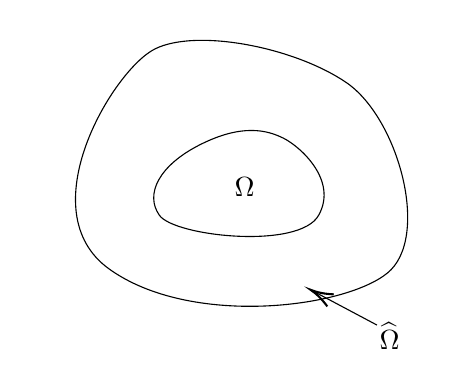
\begin{tikzpicture}[x=0.75pt,y=0.75pt,yscale=-1,xscale=1]
		%uncomment if require: \path (0,186); %set diagram left start at 0, and has height of 186
		
		%Shape: Polygon Curved [id:ds44909645306751744] 
		\draw   (106.78,9.85) .. controls (126.78,-0.15) and (173.78,8.85) .. (199,26) .. controls (224.22,43.15) and (239.78,100.85) .. (218.78,117.85) .. controls (197.78,134.85) and (123.78,143.85) .. (84.78,115.85) .. controls (45.78,87.85) and (86.78,19.85) .. (106.78,9.85) -- cycle ;
		%Shape: Polygon Curved [id:ds2016744979638545] 
		\draw   (128.78,55.85) .. controls (148.78,45.85) and (160.78,48.85) .. (168.78,52.85) .. controls (176.78,56.85) and (195,73) .. (185.78,89.85) .. controls (176.57,106.71) and (116.22,100.15) .. (109,90) .. controls (101.78,79.85) and (108.78,65.85) .. (128.78,55.85) -- cycle ;
		%Straight Lines [id:da6671306192262547] 
		\draw    (213.78,142.85) -- (183.55,126.79) ;
		\draw [shift={(181.78,125.85)}, rotate = 387.98] [color={rgb, 255:red, 0; green, 0; blue, 0 }  ][line width=0.75]    (10.93,-3.29) .. controls (6.95,-1.4) and (3.31,-0.3) .. (0,0) .. controls (3.31,0.3) and (6.95,1.4) .. (10.93,3.29)   ;
		
		% Text Node
		\draw (213.78,140.25) node [anchor=north west][inner sep=0.75pt]    {$\widehat{\Omega }$};
		% Text Node
		\draw (144,70.4) node [anchor=north west][inner sep=0.75pt]    {$\Omega $};
		
		
	\end{tikzpicture}
	
	Пусть также 
	\begin{equation*}
		\hfill\K_1(\Omega)=\left\{u|u\in\Cfn{1}(\Omega),\ u\Big|_{\partial\Omega}=0,\ \iiint\limits_{\Omega}u^2\,d\Omega=1\right\},\hfill
	\end{equation*}
	\begin{equation*}
		\hfill{\mathop{\K}\limits^0}_1(\widehat{\Omega})=\left\{u|u\in\K_1(\Omega),\ u(x,y,z)\equiv0,\ (x,y,z)\in\widehat{\Omega}\bigm\backslash\!\Omega\right\},\hfill
	\end{equation*}
	\begin{equation*}
		\K_1(\widehat{\Omega})=\left\{u|u\in\Cfn{1}\big(\widehat{\Omega}\big)\text{ --- кусочно},\ u\Big|_{\partial\widehat{\Omega}}=0,\ \iiint\limits_{\widehat{\Omega}}u^2\,d\Omega=1\right\}.
	\end{equation*}
	\begin{gather*}
		\intertext{При $u\in\K_1\big(\widehat{\Omega}\big)$  положим}\widehat{B}[u]=\iiint\limits_{\widehat{\Omega}}\Big(\left|\nabla u\right|^2+P\cdot\left|u\right|^2\Big)\,d\Omega.
	\end{gather*}
	Из определения класса $\displaystyle{\mathop{\K}\limits^0}_1\big(\widehat{\Omega}\big)$ следует, что при $u\in{\mathop{\K}\limits^0}_1\big(\widehat{\Omega}\big)$
	\begin{equation*}
		\widehat{B}[u]=B[u]=\iiint\limits_{{\Omega}}\Big(\left|\nabla u\right|^2+P\cdot\left|u\right|^2\Big)\,d\Omega.
	\end{equation*}
	Далее, для $\forall\phi\in\fLr[\widehat{\Omega}]$ положим 
	\begin{equation*}
		\check{\phi}(x,y,z)=\begin{cases}
			\phi&(x,y,z)\in\Omega,\\
			0&(x,y,z)\in\widehat{\Omega}\bigm\backslash\!\Omega.
		\end{cases}
	\end{equation*}
	Пусть $\phi_1,\ldots,\phi_k$ --- любые фиксированные функции из $\fLr[\widehat{\Omega}]$. Тогда для $u\in{\mathop{\K}\limits^0}_1(\widehat{\Omega})$ очевидно, $\big(u,\phi_j\big)_{\widehat{\Omega}}=\big(u,\check{\phi}_j\big)_{\Omega}$. Имеем
	\begin{equation}\label{l10:eq:13a}
		\hfill\begin{array}{rcl}
			\widehat{B}[u]&=&B[u],\\
			u\in{\mathop{\K}\limits^0}_1(\widehat{\Omega})& &u\in{\mathop{\K}\limits^0}_1(\widehat{\Omega}),\\
			\big(u,\phi_j\big)_{\widehat{\Omega}}=0,\ j=\overline{1,k}&  &\big(u,\check{\phi}_j\big)_{\Omega}=0,\ j=\overline{1,k}.
		\end{array}\tag{\theequation a}\hfill
	\end{equation} 
	Оставляя справа в~\eqref{l10:eq:13a} функцию $u$ фиксированной, слева возьмём минимум по $v\in\K_1\big(\widehat{\Omega}\big)\?\supseteq{\mathop{\K}\limits^0}_1(\widehat{\Omega})$. Получим
	\begin{equation}\label{l10:eq:13b}
		\hfill\begin{array}{rcl}
			\min\widehat{B}[v]&\leqslant&B[u],\\
			v\in\K_1(\widehat{\Omega})& &u\in{\mathop{\K}\limits^0}_1(\widehat{\Omega}),\\
			\big(v,\phi_j\big)_{\widehat{\Omega}}=0,\ j=\overline{1,k}&  &\big(u,\check{\phi}_j\big)_{\Omega}=0,\ j=\overline{1,k}.
		\end{array}\tag{\theequation b}\hfill
	\end{equation} 
	Так как~\eqref{l10:eq:13b} выполняется для $\forall u\in{\mathop{\K}\limits^0}_1(\widehat{\Omega})$ возьмём справа минимум по функциям $u$, причём вместо ${\mathop{\K}\limits^0}_1(\widehat{\Omega})$ возьмём $\K_1(\Omega)$.
	\begin{equation}\label{l10:eq:14}
		\hfill\begin{array}{rcl}
			\min\widehat{B}[v]&\leqslant&\min B[u],\\
			v\in\K_1(\widehat{\Omega})& &u\in\K_1(\Omega),\\
			\big(v,\phi_j\big)_{\widehat{\Omega}}=0,\ j=\overline{1,k}&  &\big(u,\check{\phi}_j\big)_{\Omega}=0,\ j=\overline{1,k}.
		\end{array}\hfill
	\end{equation} 
	Оставляя слева $\phi_1,\ldots,\phi_k$ --- фиксированными, возьмём справа в~\eqref{l10:eq:14} максимум в условии ортогональности $\big(u,\check{\phi}_j\big)_{\Omega}=0$ по всевозможным $\psi_j\in\fLr[\Omega]$. Получим
	\begin{equation}\label{l10:eq:15}
		\hfill\begin{array}{rcll}
			\min\widehat{B}[v]&\leqslant&\max&\min B[u],\\
			v\in\K_1(\widehat{\Omega})&  &\psi_1,\ldots,\psi_k &u\in\K_1(\Omega),\\
			\big(v,\phi_j\big)_{\widehat{\Omega}}=0,\ j=\overline{1,k}& &   &\big(u,\check{\psi}_j\big)_{\Omega}=0,\ j=\overline{1,k}.
		\end{array}\hfill
	\end{equation}
	А теперь возьмём в~\eqref{l10:eq:15} слева максимум по $\forall\phi_1,\ldots,\phi_k\in\fLr[\widehat{\Omega}]$. Получим окончательно
	\begin{equation}\label{l10:eq:16}
		\hfill\begin{array}{rrcll}
			\max&\min\widehat{B}[v]&\leqslant&\max&\min B[u],\\
			\phi_1,\ldots,\phi_k&v\in\K_1(\widehat{\Omega})&  &\psi_1,\ldots,\psi_k &u\in\K_1(\Omega),\\
			&\big(v,\phi_j\big)_{\widehat{\Omega}}=0,\ j=\overline{1,k} & &  &\big(u,\check{\psi}_j\big)_{\Omega}=0,\ j=\overline{1,k}.
		\end{array}\hfill
	\end{equation}	
	Согласно принципу минимакса слева в~\eqref{l10:eq:16} $\lambda_{k+1}\big(\widetilde{\Omega}\big)$, справа $\lambda_{k+1}\big(\Omega\big)$ и таким образом теорема~\ref{l10:teor:sr2} доказана, так как в~\eqref{l10:eq:16}: $\lambda_{k+1}\big(\widetilde{\Omega}\big)\leqslant\lambda_{k+1}\big(\Omega\big)$.  
\end{proof}

Возьмём теперь два произвольных куба $A_1$, $A_2$, один из которых $A_2$ содержит $\Omega$ (можно считать в теореме~\ref{l10:teor:sr2} $A_2=\widehat{\Omega}$), а другой $A_1\subset\Omega$. Пусть $\lambda_k(A_s)$ собственные значения оператора $H(A_s)$, то есть оператора $H$в кубе $A_s$ с нулевым граничным условием на $\partial A_s$, $s=1,2$. В силу теоремы~\ref{l10:teor:sr2}
\begin{equation}\label{l10:eq:1.17}
	\lambda_k(A_1)\geqslant\lambda_k\geqslant\lambda_k(A_2).
\end{equation}
Пусть $P_{+}^{(1)}=\max\limits_{r\in A_1}P(r)$, $P_{-}^{(2)}=\min\limits_{r\in A_2}P(r)$ $r=(x,y,z)$ и $\lambda_k^{+}(A_1)$, $\lambda_k^{-}(A_2)$ --- собственные значения операторов $H_{+}(A_1)=-\Delta+P_{+}^{(1)}$ и $H_{-}(A_2)=-\Delta+P_{-}^{(2)}$ в кубах $A_1$, $A_2$ с нулевым условием на $\partial A_1$, $\partial A_2$. Тогда в силу теоремы~\ref{l10:teor:sr1}
\begin{equation*}
	\lambda_k^{+}(A_1)\geqslant\lambda_k(A_1),\quad\lambda_k^{-}(A_2)\leqslant\lambda_k(A_2)
\end{equation*} 
и в силу~\eqref{l10:eq:1.17}
\begin{equation*}
	\lambda_k^{+}(A_1)\geqslant\lambda_k\geqslant\lambda_k^{-}(A_2),
\end{equation*} 
но для любого куба $A$ собственные значения $\lambda_k^0(A)$ оператора $H_0(A)=-\Delta+P_0$, где $P_0$ произвольная константа, известны\footnote{Мы покажем далее в курсе, что для куба $A$ со стороной $l$ собственные значения оператора $H_0(A)=-\Delta+P_0$ при нулевом граничном условии на $\partial A$ суть $\displaystyle\nu_{k_1 k_2 k_3}=\left(\frac{\pi}{l}\right)^2\cdot\left(k_1^2+k_2^2+k_3^2\right)+P_0$, где $k_1,\ k_2\ k_3=1,2,3,\ldots$. Мы упорядочиваем их по величине $\left(k_1^2+k_2^2+k_3^2\right)$ и обозначаем $\lambda_k^0(A)$.}  и $\lambda_k^0\to+\infty$ при $k\to\infty$. Значит $\lambda_k\to+\infty$ при $k\to\infty$, что мы и хотели доказать.
%Пусть $\nu_k^{(2)}$ и $\nu_k^{(1)}$ --- собственные значения оператора $H_0=-\Delta$ в $A_2$ и $A_1$ с нулевым граничным условием на $\partial A_2$ и $\partial A_1$ соответственно. В силу теоремы~\ref{l10:teor:sr2} 
%\begin{equation}\label{l10:eq:17}
%	\hfill\nu_k^{(1)}\geqslant\lambda_k\geqslant\nu_k^{(2)}.\hfill	
%\end{equation}
%Но для кубов собственные значения находятся в явном виде\footnote{Мы покажем далее в курсе, что для куба $A$ со стороной $l$ собственные значения оператора $H_0(A)=-\Delta+P_0$ при нулевом граничном условии на $\partial A$ суть $\displaystyle\nu_{k_1 k_2 k_3}=\left(\frac{\pi}{l}\right)^2\cdot\left(k_1^2+k_2^2+k_3^2\right)+P_0$, где $k_1,\ k_2\ k_3=1,2,3,\ldots$. Мы упорядочиваем их по величине $\left(k_1^2+k_2^2+k_3^2\right)$ и обозначаем $\lambda_k^0(A)$.} и для некоторых $\alpha_j>0$, $j=1,2$
%\begin{equation}\label{l10:eq:18}
%	\hfill\nu_k^{(1)}\leqslant\alpha_1\cdot k^2,\quad\nu_k^{(2)}\geqslant\alpha_2\cdot k^2.\hfill
%\end{equation}
%Поэтому в силу~\eqref{l10:eq:12a} $\displaystyle\left(\lambda_k^{-}\leqslant\lambda_k\leqslant\lambda_k^{+}\right)$  и~\eqref{l10:eq:12b} $\displaystyle\left(\lambda_k^{\pm}=\lambda_k^0+P_{\pm}\right)$ мы получаем, используя~\eqref{l10:eq:17},~\eqref{l10:eq:18} 
%\begin{equation*}
%	\hfill\alpha_2\cdot k^2+P_{-}\leqslant\lambda_k^{0}+P_{-}\leqslant\lambda_k\leqslant\lambda_k^{0}+P_{+}\leqslant\alpha_1\cdot k^2+P_{+}.\hfill
%\end{equation*}
%
%Таким образом мы получили, что собственные значения $\lambda_k$ оператора Шредингера $H=-\Delta+P$ в $\Omega$ растут со скоростью $k^2$. 

Теперь переходим к теореме Стеклова. Пусть $u_1,\ u_2,\ldots,u_k,\ldots$ --- ортонормированные собственные функции оператора Шредингера в области $\Omega$ с нулевыми условиями на $\partial\Omega$ и пусть $\lambda_1<\lambda_2\leqslant\ldots\leqslant\lambda_k\leqslant\ldots$ соответствующие собственныые значения, $C_k=\big(u,u_k\big)$, $u\in\fLr[\Omega]$. 
\begin{_teor}[Стеклова]\hfill
	\begin{enumerate1}
		\item\label{l10:Steclov:1} Для любой функции $u\in\fLr[\Omega]$ обобщённый ряд Фурье $\displaystyle\sum\limits_{k=1}^{\infty}C_k\cdot u_k$ сходится к $u$ в среднем.
		\item\label{l10:Steclov:2} Для любой функции $u\in\mc{D}_{H}$ ряд  $\displaystyle\sum\limits_{k=1}^{\infty}C_k\cdot u_k$ сходится к ней равномерно.
	\end{enumerate1}
\end{_teor}
Утверждение~\ref{l10:Steclov:1} доказывается так же, как в одномерном случае. Сначала показывается, что при $u\in\mc{D}_H$ выполняется $\norm{u-S_n}\to0$, а затем без доказательства используем, что для $\forall u\?\in\fLr[\Omega]$ по $\forall\eps>0$ $\exists u_{\eps}\in\mc{D}_H$ так, что $\norm{u-u_{\eps}}<\eps$. Утверждение~\ref{l10:Steclov:2} теоремы Стеклова --- без доказательства.

\section{Различные обобщения.}
\label{lecture10section2}
\subsection{Оператор Штурма. Случай периодических граничных условий.}
\label{lecture10section2sub1}
Пусть
\begin{equation*}
	\hfill Ly=-\der{}{x}\Big(Q\cdot y'\Big)+P\cdot y,\quad\mc{D}_{L}=\left\{y|y\in\Cfn[{[a,b]}]{2},\ y(a)=y(b),\ y'(a)=y'(b)\right\}_{\displaystyle.}\hfill
\end{equation*}
Легко проверить, что при $Q(a)=Q(b)$ оператор $L$ --- эрмитов и значит собственные значения вещественны и собственные функции, отвечающие различным собственным значениям взаимно ортогональны. Есть отличие от рассмотренных нами ранее ситуаций; отличие, которое нам подсказывает оператор
\begin{equation*}
	\hfill Ly=-\dder{}{x}y\quad\text{при }[a,b]=[0,l].\hfill
\end{equation*}
Мы получаем собственные значения $\displaystyle\lambda_k=\left(\frac{2\cdot\pi\cdot k}{l}\right)^2$ и собственные функции (две!), отвечающие каждому собственному значению $\lambda_k\neq0$
\begin{equation*}
	\hfill y_{k1}=\sqrt{\frac{2}{l}}\cdot\sin\left(\frac{2\cdot\pi\cdot k}{l}\cdot x\right),\quad y_{k2}=\sqrt{\frac{2}{l}}\cdot\cos\left(\frac{2\cdot\pi\cdot k}{l}\cdot x\right),\quad y_0=\frac{1}{\sqrt{l}}.\hfill
\end{equation*}
В остальном --- доказательство свойств оператора Штурма с периодическими граничными условиями не отличается от проведённого для обычного оператора Штурма при условиях $y(a)=y(b)\?=0$. Заметим только, что при $l=2\cdot\pi$ мы в теореме Стеклова получили разложение в обычный ряд Фурье.
\subsection{Случай неограниченной области.} 
\label{lecture10section2sub2}
Рассмотрим оператор $Ly=-y''$ на полуоси $[0,+\infty)$ в пространстве $\fL[{[0,+\infty)}]$, с заданным условием $y(0)=0$ и условием $\smallint\limits_0^{\infty}|y'|^2\,dx<+\infty$, заменяющим условие на бесконечности. 

Тогда если $-y''=\lambda\cdot y$, то $y''\in\fL[{[0,\infty)}]$. Найдём знак $\lambda$. Пусть $N\gg1$
\begin{equation*}
	-\underline{\int\limits_0^N y''\cdot\overline{y}\,dx}=-y'\cdot\overline{y}\mathop{\Big|}\limits_{0}^{N}+\underline{\int\limits_0^N|y'|^2\,dx}=-y'\cdot\overline{y}\Big|_{x=N}+\underline{\int\limits_0^N|y'|^2\,dx}=\lambda\cdot\underline{\int\limits_0^N|y|^2\,dx}.
\end{equation*}    
При $N\to\infty$ подчёркнутые интегралы имеют конечный предел, значит и $\alpha=\lim\limits_{N\to\infty}y'(N)\cdot y(N)$ --- существует и конечен. Но так как интеграл  $\smallint\limits_0^{\infty}|y'\cdot y|\,dx$ --- конечен, то $\alpha=0$ и поэтому в пределе при $N\to\infty$ мы получаем, что
\begin{equation*}
	\hfill\int\limits_0^{\infty}|y'|^2\,dx=\lambda\cdot\int\limits_0^{\infty}y^2\,dx.\hfill
\end{equation*}
Значит $\lambda\geqslant0$. Полагая $\lambda=\nu^2$ из условия $-y''=\nu^2\cdot y$ находим $y=c_1\cdot\sin\left(\nu\cdot x\right)$. Но $y\notin\fL[{[0,\infty)}]$, хотя формально удовлетворяет уравнению $-y''=\nu^2\cdot y$. Таким образом у рассматриваемого оператора в $\fL[{[0,\infty)}]$ нет собственных функций. Поэтому в привычном виде нет теоремы Стеклова. В то же время, если $y\in\fL[{[0,\infty)}]\cap\fLone[{[0,\infty)}]$\footnote{$\displaystyle\fLone[{[0,\infty)}]=\left\{y(x)|\int\limits_{0}^{\infty}|y(x)|\,dx<+\infty\right\}_{\displaystyle.}$} то для 
\begin{equation*}
	\hfill \overline{y}(\nu)\eqdef\int\limits_0^{\infty}y(x)\cdot\sin\left(\nu\cdot x\right)\,dx\hfill
\end{equation*}
имеет место 
\begin{equation*}
	\hfill y(x)=\frac{1}{\pi}\cdot\int\limits_0^{\infty}\overline{y}(\nu)\cdot\sin\left(\nu\cdot x\right)\,d\nu.\hfill
\end{equation*}
Здесь $\overline{y}(\nu)$ --- это не комплексно сопряжённая функция, а обозначение\footnote{Приведённые формулы относятся к синус-преобразованию, которое мы будем изучать в последних лекциях.}.
Функция $\sin\left(\nu\cdot x\right)$ называется собственной функцией непрерывного спектра, $\overline{y}(\nu)$ --- аналог коэффициента Фурье. Если рассмотреть на полуоси оператор 
\begin{equation*}
	Ly=-y''+P(x)\cdot y,\quad P(x)\to0,\ x\to\infty,
\end{equation*}
тогда может быть какое-то число собственных значений $\lambda_n$. Пусть собственные функции суть $y_n(x)$ тогда
\begin{equation*}
	\hfill y(x)=\sum\limits_{n}C_n\cdot y_n+\int\dots\,.\hfill
\end{equation*}
\section{Оператор Шредингера во всём пространстве.}
\label{lecture10section3}
Поскольку такие операторы встречаются в квантовой механике, то мы будем обсуждать ситуацию применительно к ней.
\subsection{Одночастичный случай.}
\label{lecture10section3sub1}
Пусть $\bm{r}=(x,y,z)$, оператор энергии
\begin{equation*}
	\hfill Hu=-a\cdot\Delta u+P(\bm{r})\cdot u.\hfill
\end{equation*}
Область определения
\begin{equation*}
	\hfill\mc{D}_{H}=\left\{u(\bm{r})|u\in\Cfn{2}\big(\R^3\big),\ \iiint\limits_{\R^3}\left(|u|^2+|\nabla u|^2\right)\,d\Omega<+\infty,\ Hu\in\fLr[\R^3]\right\}_{\displaystyle.}\hfill
\end{equation*}
Пример:
\begin{equation*}
	\hfill Hu=-a\cdot\Delta u-\frac{1}{|\bm{r}|}\cdot u\text{ --- гамильтониан атома водорода.}\hfill
\end{equation*}
В общем случае
\begin{equation*}
	\hfill Hu=-a\cdot\Delta u+P(\bm{r})\cdot u,\ P(\bm{r})\to0\text{ при }|\bm{r}|\to\infty.\hfill
\end{equation*} 
Для простоты считаем, что $P(\bm{r})<0$ при $|\bm{r}|\gg1$. Тогда доказано, что если $|\bm{r}|^2\cdot|P(\bm{r})|\to0$ при $|\bm{r}|\to\infty$, то слева от точки $0$ может быть не более чем конечное число собственных значений. Это так называемые короткодействующие взаимодействия $P(\bm{r})$, характерные для взаимодействий между нуклонами. Если $|\bm{r}|^2\cdot|P(\bm{r})|\to+\infty$	при $|\bm{r}|\to\infty$ --- то это --- длиннодействие. Пример $P(\bm{r})=-\dfrac{c}{|\bm{r}|} (c>0)$ --- случай атома водорода. При отрицательном длиннодействии имеется бесконечное число собственных значений $\lambda_k<0$, $\lambda_k\to0$, $k\to\infty$.
\vspace{0.2cm}

\tikzset{every picture/.style={line width=0.75pt}} %set default line width to 0.75pt        

\begin{tikzpicture}[x=0.75pt,y=0.75pt,yscale=-1,xscale=1]
	%uncomment if require: \path (0,164); %set diagram left start at 0, and has height of 164
	
	%Straight Lines [id:da9857502589663749] 
	\draw  [dash pattern={on 0.84pt off 2.51pt}]  (41,71) -- (125.78,71) ;
	%Straight Lines [id:da29507301408727105] 
	\draw    (125.78,71) -- (280.78,71) ;
	%Shape: Circle [id:dp15804261182116908] 
	\draw  [fill={rgb, 255:red, 0; green, 0; blue, 0 }  ,fill opacity=1 ] (122.17,71) .. controls (122.17,69.01) and (123.79,67.39) .. (125.78,67.39) .. controls (127.78,67.39) and (129.39,69.01) .. (129.39,71) .. controls (129.39,72.99) and (127.78,74.61) .. (125.78,74.61) .. controls (123.79,74.61) and (122.17,72.99) .. (122.17,71) -- cycle ;
	
	% Text Node
	\draw (49,49.4) node [anchor=north west][inner sep=0.75pt]    {$\lambda _{k}$};
	% Text Node
	\draw (121,49.4) node [anchor=north west][inner sep=0.75pt]    {$0$};
	
	
\end{tikzpicture}
\vspace{0.2cm}

\noindent В обоих случаях ось $[0,+\infty)$ заполнена <<непрерывным спектром>> --- то есть точкам $\nu>0$ отвечают не интегрируемые с квадратом собственные функции и теорема Стеклова будет выглядеть так
\begin{equation*}
	\hfill u(x)=\sum\limits_{k}C_k\cdot u_k+\iiint\dots\,.\hfill 
\end{equation*} 




А если $P(\bm{r})\to+\infty$ $|\bm{r}|\to\infty$ то у оператора $H$ не будет непрерывного спектра, собственные значения $\lambda_k\to+\infty$ и теорема Стеклова справедлива в обычной формулировке. 
\subsection{Многоэлектронный атом с неподвижным ядром.}
\label{lecture10section3sub2}
Оператор энергии $n$-электронного атома
\begin{equation*}
	\hfill H_n u=-\sum\limits_{i=1}^{n}a\cdot\Delta_i u-Z\cdot e^2\cdot\sum\limits_{i=1}^{n}\frac{1}{|\bm{r}_i|}\cdot u+e^2\cdot\sum\limits_{\substack{i,j=1\\ i<j}}^n\frac{1}{|\bm{r}_{ij}|}\cdot u,\hfill
\end{equation*}
где $\displaystyle u=u(\bm{r}_1,\ldots,\bm{r}_n)$, $\displaystyle \bm{r}_i=(x_i,y_i,z_i)$ --- координаты $i$-ого электрона, $\displaystyle |Z\cdot e|$ --- заряд ядра, $e$ --- заряд электрона, $\displaystyle \bm{r}_{ij}=\bm{r}_i-\bm{r}_j$, $\displaystyle\Delta_i=\pdder{}{x_i}+\pdder{}{y_i}+\pdder{}{z_i}$. Для нейтрального атома $Z=n$, для $(+)$ иона $Z>n$.
\begin{equation*}
	\hfill\mc{D}_{H_n}=\left\{u(\bm{r}_1,\ldots,\bm{r}_n)|u\in\Cfn{2}\left(\R^{3\cdot n}\right)\text{ --- кусочно},\ \idotsint\limits_{\R^{3\cdot n}}\left(|u|^2+\left|\nabla u\right|^2+\left|Hu\right|^2\right)\,d\Omega<+\infty\right\}_{\displaystyle.}\hfill
\end{equation*}
Уравнение
\begin{equation*}
	\hfill H_n u=\lambda\cdot u\hfill
\end{equation*}
описывает стационарные (связанные) состояния атома (иона) с энергией $\lambda$. Хотя написанное уравнение является одним из основных уравнений не релятивистской квантовой механики, вопрос о существовании собственных значений, их числе и местоположении не был решён к $60^{\text{\underline{м}}}$ годам прошлого века. Задача исследования этого вопроса была поставлена мне в аспирантуре (1956-1959). Результаты решения этой задачи привожу ниже. При $Z\geqslant n$ (случай нейтральных атомов ($Z=n$) и положительных ионов ($Z>n$)) существует бесконечная серия собственных значений $\lambda_k(n)\to\lambda_{0}(n-1)$ при $k\to\infty$, где $\lambda_0(n-1)$ --- наименьшее собственное значение оператора $H_{n-1}$, то есть при $Z=n$ нижняя грань энергии $(+)$ иона, получившегося удалением из системы одного электрона (теорема Жислина). Сплошной спектр заполняет луч $\big[\lambda_0(n-1),+\infty\big)$ (HWZ--theorem, теорема Хунцикера--ван Винтера--Жислина).
\vspace{0.5cm}



\tikzset{every picture/.style={line width=0.75pt}} %set default line width to 0.75pt        

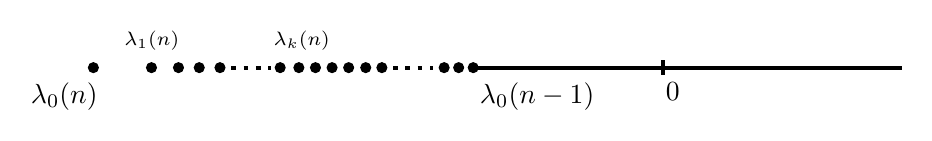
\begin{tikzpicture}[x=0.75pt,y=0.75pt,yscale=-1,xscale=1]
	%uncomment if require: \path (0,100); %set diagram left start at 0, and has height of 100
	
	%Shape: Circle [id:dp35029628015737635] 
	\draw  [fill={rgb, 255:red, 0; green, 0; blue, 0 }  ,fill opacity=1 ] (91,41.39) .. controls (91,40.07) and (92.07,39) .. (93.39,39) .. controls (94.71,39) and (95.78,40.07) .. (95.78,41.39) .. controls (95.78,42.71) and (94.71,43.78) .. (93.39,43.78) .. controls (92.07,43.78) and (91,42.71) .. (91,41.39) -- cycle ;
	%Shape: Circle [id:dp1287901849890314] 
	\draw  [fill={rgb, 255:red, 0; green, 0; blue, 0 }  ,fill opacity=1 ] (63,41.39) .. controls (63,40.07) and (64.07,39) .. (65.39,39) .. controls (66.71,39) and (67.78,40.07) .. (67.78,41.39) .. controls (67.78,42.71) and (66.71,43.78) .. (65.39,43.78) .. controls (64.07,43.78) and (63,42.71) .. (63,41.39) -- cycle ;
	%Shape: Circle [id:dp2709087999318953] 
	\draw  [fill={rgb, 255:red, 0; green, 0; blue, 0 }  ,fill opacity=1 ] (104,41.39) .. controls (104,40.07) and (105.07,39) .. (106.39,39) .. controls (107.71,39) and (108.78,40.07) .. (108.78,41.39) .. controls (108.78,42.71) and (107.71,43.78) .. (106.39,43.78) .. controls (105.07,43.78) and (104,42.71) .. (104,41.39) -- cycle ;
	%Shape: Circle [id:dp2466500958363409] 
	\draw  [fill={rgb, 255:red, 0; green, 0; blue, 0 }  ,fill opacity=1 ] (114,41.39) .. controls (114,40.07) and (115.07,39) .. (116.39,39) .. controls (117.71,39) and (118.78,40.07) .. (118.78,41.39) .. controls (118.78,42.71) and (117.71,43.78) .. (116.39,43.78) .. controls (115.07,43.78) and (114,42.71) .. (114,41.39) -- cycle ;
	%Shape: Circle [id:dp5728346002535216] 
	\draw  [fill={rgb, 255:red, 0; green, 0; blue, 0 }  ,fill opacity=1 ] (124,41.39) .. controls (124,40.07) and (125.07,39) .. (126.39,39) .. controls (127.71,39) and (128.78,40.07) .. (128.78,41.39) .. controls (128.78,42.71) and (127.71,43.78) .. (126.39,43.78) .. controls (125.07,43.78) and (124,42.71) .. (124,41.39) -- cycle ;
	%Shape: Circle [id:dp6861896993895451] 
	\draw  [fill={rgb, 255:red, 0; green, 0; blue, 0 }  ,fill opacity=1 ] (153,41.39) .. controls (153,40.07) and (154.07,39) .. (155.39,39) .. controls (156.71,39) and (157.78,40.07) .. (157.78,41.39) .. controls (157.78,42.71) and (156.71,43.78) .. (155.39,43.78) .. controls (154.07,43.78) and (153,42.71) .. (153,41.39) -- cycle ;
	%Shape: Circle [id:dp3925876580198855] 
	\draw  [fill={rgb, 255:red, 0; green, 0; blue, 0 }  ,fill opacity=1 ] (162,41.39) .. controls (162,40.07) and (163.07,39) .. (164.39,39) .. controls (165.71,39) and (166.78,40.07) .. (166.78,41.39) .. controls (166.78,42.71) and (165.71,43.78) .. (164.39,43.78) .. controls (163.07,43.78) and (162,42.71) .. (162,41.39) -- cycle ;
	%Shape: Circle [id:dp6339036403733711] 
	\draw  [fill={rgb, 255:red, 0; green, 0; blue, 0 }  ,fill opacity=1 ] (170,41.39) .. controls (170,40.07) and (171.07,39) .. (172.39,39) .. controls (173.71,39) and (174.78,40.07) .. (174.78,41.39) .. controls (174.78,42.71) and (173.71,43.78) .. (172.39,43.78) .. controls (171.07,43.78) and (170,42.71) .. (170,41.39) -- cycle ;
	%Shape: Circle [id:dp8399524505957763] 
	\draw  [fill={rgb, 255:red, 0; green, 0; blue, 0 }  ,fill opacity=1 ] (178,41.39) .. controls (178,40.07) and (179.07,39) .. (180.39,39) .. controls (181.71,39) and (182.78,40.07) .. (182.78,41.39) .. controls (182.78,42.71) and (181.71,43.78) .. (180.39,43.78) .. controls (179.07,43.78) and (178,42.71) .. (178,41.39) -- cycle ;
	%Shape: Circle [id:dp9411154337862653] 
	\draw  [fill={rgb, 255:red, 0; green, 0; blue, 0 }  ,fill opacity=1 ] (186,41.39) .. controls (186,40.07) and (187.07,39) .. (188.39,39) .. controls (189.71,39) and (190.78,40.07) .. (190.78,41.39) .. controls (190.78,42.71) and (189.71,43.78) .. (188.39,43.78) .. controls (187.07,43.78) and (186,42.71) .. (186,41.39) -- cycle ;
	%Shape: Circle [id:dp2552161753644939] 
	\draw  [fill={rgb, 255:red, 0; green, 0; blue, 0 }  ,fill opacity=1 ] (194.22,41.39) .. controls (194.22,40.07) and (195.29,39) .. (196.61,39) .. controls (197.93,39) and (199,40.07) .. (199,41.39) .. controls (199,42.71) and (197.93,43.78) .. (196.61,43.78) .. controls (195.29,43.78) and (194.22,42.71) .. (194.22,41.39) -- cycle ;
	%Shape: Circle [id:dp24926192241913614] 
	\draw  [fill={rgb, 255:red, 0; green, 0; blue, 0 }  ,fill opacity=1 ] (202,41.39) .. controls (202,40.07) and (203.07,39) .. (204.39,39) .. controls (205.71,39) and (206.78,40.07) .. (206.78,41.39) .. controls (206.78,42.71) and (205.71,43.78) .. (204.39,43.78) .. controls (203.07,43.78) and (202,42.71) .. (202,41.39) -- cycle ;
	%Shape: Circle [id:dp1350201796938677] 
	\draw  [fill={rgb, 255:red, 0; green, 0; blue, 0 }  ,fill opacity=1 ] (232,41.39) .. controls (232,40.07) and (233.07,39) .. (234.39,39) .. controls (235.71,39) and (236.78,40.07) .. (236.78,41.39) .. controls (236.78,42.71) and (235.71,43.78) .. (234.39,43.78) .. controls (233.07,43.78) and (232,42.71) .. (232,41.39) -- cycle ;
	%Shape: Circle [id:dp8879498234303822] 
	\draw  [fill={rgb, 255:red, 0; green, 0; blue, 0 }  ,fill opacity=1 ] (239,41.39) .. controls (239,40.07) and (240.07,39) .. (241.39,39) .. controls (242.71,39) and (243.78,40.07) .. (243.78,41.39) .. controls (243.78,42.71) and (242.71,43.78) .. (241.39,43.78) .. controls (240.07,43.78) and (239,42.71) .. (239,41.39) -- cycle ;
	%Shape: Circle [id:dp19584404858089832] 
	\draw  [fill={rgb, 255:red, 0; green, 0; blue, 0 }  ,fill opacity=1 ] (246,41.39) .. controls (246,40.07) and (247.07,39) .. (248.39,39) .. controls (249.71,39) and (250.78,40.07) .. (250.78,41.39) .. controls (250.78,42.71) and (249.71,43.78) .. (248.39,43.78) .. controls (247.07,43.78) and (246,42.71) .. (246,41.39) -- cycle ;
	%Straight Lines [id:da8364806346935474] 
	\draw [line width=1.5]  [dash pattern={on 1.69pt off 2.76pt}]  (131.8,41.5) -- (150.8,41.5) ;
	%Straight Lines [id:da3144831530966994] 
	\draw [line width=1.5]  [dash pattern={on 1.69pt off 2.76pt}]  (209.78,41.5) -- (228.78,41.5) ;
	%Straight Lines [id:da6689632878279683] 
	\draw [line width=1.5]    (248.39,41.39) -- (454.78,41.39) ;
	%Straight Lines [id:da12357539080200586] 
	\draw [line width=1.5]    (340,37.85) -- (340,45) ;
	
	% Text Node
	\draw (34,47.4) node [anchor=north west][inner sep=0.75pt]  [font=\normalsize]  {$\lambda _{0}( n)$};
	% Text Node
	\draw (79,22.4) node [anchor=north west][inner sep=0.75pt]  [font=\scriptsize]  {$\lambda _{1}( n)$};
	% Text Node
	\draw (151,22.4) node [anchor=north west][inner sep=0.75pt]  [font=\scriptsize]  {$\lambda _{k}( n)$};
	% Text Node
	\draw (250.39,47.18) node [anchor=north west][inner sep=0.75pt]  [font=\normalsize]  {$\lambda _{0}( n-1)$};
	% Text Node
	\draw (340,47.2) node [anchor=north west][inner sep=0.75pt]    {$0$};
	
	
\end{tikzpicture}